\documentclass[a5paper,english,spanish,brazil]{ufsc-thesis}

% ---
% PACOTES
% ---

% ---
% Pacotes fundamentais 
% ---
%\usepackage{lmodern}			% Usa a fonte Latin Modern			
\usepackage[T1]{fontenc}		% Selecao de codigos de fonte.
\usepackage[utf8]{inputenc}		% Codificacao do documento (conversão automática dos acentos)
\usepackage{lastpage}			% Usado pela Ficha catalográfica
\usepackage{indentfirst}		% Indenta o primeiro parágrafo de cada seção.
\usepackage{color}				% Controle das cores
\usepackage{graphicx}			% Inclusão de gráficos
\usepackage{subfig}  %usar duas figurasna mesma figura
\usepackage{microtype} 			% para melhorias de justificação
\usepackage{mathtools} %para usar equations
\usepackage{xfrac} %para usar \sfrac
\everymath{\displaystyle} %força todas as expressões nem estilo de maior fonte
%\usepackage{pslatex} % Coloca as letras em Times New Roman, mas não nos Títulos de seções e Capítulos 
\usepackage{listings}
\usepackage{listingsutf8}

\usepackage{longtable}
\usepackage{tabularx}

\usepackage{varioref}
\usepackage{hyperref}
\usepackage{cleveref}

\graphicspath{{figuras/}}
% ---
		
% ---
% Pacotes adicionais, usados apenas no âmbito do Modelo Canônico do abnteX2
% ---
\usepackage{lipsum}				% para geração de dummy text
% ---

% ---
% Pacotes de citações
% ---
\usepackage[brazilian,hyperpageref]{backref}	 % Paginas com as citações na bibl
\usepackage[alf]{abntex2cite}	% Citações padrão ABNT


% ---
% Informações de dados para CAPA e FOLHA DE ROSTO
% ---
\titulo{Repotencialização em Subestações de Alta Tensão Utilizando Módulos de Manobra Híbridos Compactos}
\autor{Joan Francisco {}Alvarez Burgos}
\local{Florianópolios, SC-Brasil}
\data{\today}
\orientador{Maurício Valencia {}Ferreira da Luz}
%\coorientador{Equipe \abnTeX}
%\instituicao{
%  Universidade Federal de Santa Catarina -- UFSC
%  \par
%  Centro Tecnológico -- CTC
%  \par
%  Departamento de Engenharia Elétrica -- EEL}
\instituicao{Universidade Federal de Santa Catarina}
\centro{Centro Tecnológico -- CTC}
\programa{Programa de Graduação em Engenharia Elétrica}
\assuntos{Subestações,Sistemas de Potência,Instalações Elétricas,Orçamentos}
\tipotrabalho{Trabalho de Conclusão de Curso}
% O preambulo deve conter o tipo do trabalho, o objetivo, 
% o nome da instituição e a área de concentração 
\preambulo{Monografia submetida ao Programa de Graduação em Engenharia Elétrica da Universidade Federal de Santa Catarina como requisito para aprovação na disciplina EEL7890 -- Trabalho de Conclusão de Curso (TCC).}
% ---


% ---
% Configurações de aparência do PDF final

% alterando o aspecto da cor azul
\definecolor{blue}{RGB}{6,69,173} %padrão wikipedia de cor de link

% informações do PDF
\makeatletter
\hypersetup{
     	%pagebackref=true,
		pdftitle={\@title}, 
		pdfauthor={\@author},
    	pdfsubject={\imprimirpreambulo},
	    pdfcreator={LaTeX with abnTeX2},
		pdfkeywords={abnt}{latex}{abntex}{abntex2}{trabalho acadêmico}, 
		colorlinks=true,       		% false: boxed links; true: colored links
    	linkcolor=blue,          	% color of internal links
    	citecolor=blue,        		% color of links to bibliography
    	filecolor=magenta,      		% color of file links
		urlcolor=blue,
		bookmarksdepth=4
}
\makeatother
% --- 

% --- 
% Espaçamentos entre linhas e parágrafos 
% --- 

% O tamanho do parágrafo é dado por:
%\setlength{\parindent}{1.3cm}

% Controle do espaçamento entre um parágrafo e outro:
%\setlength{\parskip}{0.2cm}  % tente também \onelineskip

% ---
% compila o indice
% ---
\makeindex
% ---

% ----
% Início do documento
% ----
\begin{document}
% Retira espaço extra obsoleto entre as frases.
\frenchspacing 

% ----------------------------------------------------------
% ELEMENTOS PRÉ-TEXTUAIS
% ----------------------------------------------------------
\pretextual

% ---
% Capa
% ---
\imprimircapa
% ---

% ---
% Folha de rosto
% (o * indica que haverá a ficha bibliográfica)
% ---
\imprimirfolhaderosto*
% ---

%\clearpage
\imprimirfichacatalografica

% ---
% Inserir folha de aprovação
% ---

% Isto é um exemplo de Folha de aprovação, elemento obrigatório da NBR
% 14724/2011 (seção 4.2.1.3). Você pode utilizar este modelo até a aprovação
% do trabalho. Após isso, substitua todo o conteúdo deste arquivo por uma
% imagem da página assinada pela banca com o comando abaixo:
%
% \includepdf{folhadeaprovacao_final.pdf}
%
\begin{folhadeaprovacao}

  \begin{center}
    {\imprimirautor}

    \vspace*{\fill}\vspace*{\fill}
    \begin{center}
      \ABNTEXchapterfont\bfseries\Large\imprimirtitulo
    \end{center}
    \vspace*{\fill}
    
    %\hspace{.45\textwidth}
    
    	\begin{center}
    		\vspace*{0.5cm}
    		Esta Monografia foi julgada no contexto da disciplina EEL7890 -- Trabalho de Conclusão de Curso (TCC), e aprovado em sua forma final pelo Programa de Engenharia Elétrica da Universidade Federal de Santa Catarina.
    		\vspace*{0.5cm}
  		\end{center}
    
    \vspace*{\fill}
   \end{center}
  
  \begin{center}
    %\vspace*{0.5cm}
    {\large\imprimirlocal},
    {\large\imprimirdata}
    %\vspace*{1cm}
  \end{center}
        
   \assinatura{\textbf{ Prof. Dr. Eng. Renato Lucas Pacheco} \\ Coordenador de Graduação}
   Banca Examinadora:
   \assinatura{\textbf{Prof. Dr. Eng. \imprimirorientador} \\ Orientador} 
   \assinatura{\textbf{Professor} \\ Convidado 1}
   \assinatura{\textbf{Professor} \\ Convidado 2}
   %\assinatura{\textbf{Professor} \\ Convidado 3}
   %\assinatura{\textbf{Professor} \\ Convidado 4}
      

\end{folhadeaprovacao}
% ---

% ---
% Dedicatória
% ---
\begin{dedicatoria}
   \vspace*{\fill}
   \centering
   \noindent
   \textit{Este trabalho é dedicado à minha família que foram tão compreensíveis e me deram tanto apoio nos momentos difíceis da jornada da graduação} \vspace*{\fill}
\end{dedicatoria}
% ---

% ---
% Agradecimentos
% ---
\begin{agradecimentos}
\lipsum[1]
\end{agradecimentos}
% ---

% ---
% Epígrafe
% ---
\begin{epigrafe}
    \vspace*{\fill}
		\noindent
		\hangindent=5cm \\
  \textit{`` O homem disse que tinha de ir embora -- antes queria me ensinar uma coisa muito importante: -- Você quer conhecer o segredo de ser um menino feliz para o resto da sua vida? \\ -- Quero -- Respondi. \\ O segredo se resume em três palavras, que ele pronunciou com intensidade, mãos nos meus ombros e olhos nos meus olhos: \\ -- Pense nos outros.''}
    \begin{flushright}
		Fernando Sabino	
		\end{flushright}		
\end{epigrafe}
% ---

% ---
% RESUMOS
% ---

% resumo em português
%\setlength{\absparsep}{18pt} % ajusta o espaçamento dos parágrafos do resumo
%\begin{resumo}
%Aqui vai o resumo

% \textbf{Palavras-chaves}: latex. abntex. editoração de texto.
%\end{resumo}

% resumo em inglês
%\begin{resumo}[Abstract]
% \begin{otherlanguage*}{english}
%   This is the english abstract.

%   \vspace{\onelineskip}
 
%   \noindent 
%   \textbf{Key-words}: latex. abntex. text editoration.
% \end{otherlanguage*}
%\end{resumo}


% ---
% inserir lista de ilustrações
% ---
%\pdfbookmark[0]{\listfigurename}{lof}
\listoffigures
\cleardoublepage
% ---

% ---
% inserir lista de tabelas
% ---
%\pdfbookmark[0]{\listtablename}{lot}
\listoftables*
\cleardoublepage
% ---

% ---
% inserir lista de abreviaturas e siglas
% ---
\begin{siglas}
  \item[Celesc] Centrais Elétricas de Santa Catarina
  \item[SE] Subestação
  \item[CBU] Camboriú
  \item[CMB] Camboriú Morro do Boi
\end{siglas}
% ---

% ---
% inserir lista de símbolos
% ---
\begin{simbolos}
  \item[$ \Omega $] Letra grega Ômega
  \item[$ \Delta $] Letra grega Delta
\end{simbolos}

% ---
% inserir o sumario
% ---
\pdfbookmark[0]{\contentsname}{toc}
\tableofcontents*
\cleardoublepage
% ---

% ----------------------------------------------------------
% ELEMENTOS TEXTUAIS
% ----------------------------------------------------------
\textual %isto faz as páginas dos elementos textuais serem numeradas

% ----------------------------------------------------------
% Introdução
% ----------------------------------------------------------
%\chapter*[Introdução]{Introdução} %o asterisco exclui a numeração e retira do sumário
%\addcontentsline{toc}{chapter}{Introdução} %este volta a adicionar ao sumário a introdução
\chapter{Introdução}
O estudo de caso consiste na ampliação da Subestação Camboriú de responsabilidade das Centrais Elétricas de Santa Catarina – Celesc que opera em plena carga de 30MVA segundo dados do Centro de Operação do Sistema Elétrico da Celesc desde final de 2013.

\section{Motivação}
O acadêmico teve a possibilidade de realizar o programa de estágio na empresa Celesc Distribuição S.A. na Divisão de Subestações que possibilitou o contato com projetos de todo o estado de Santa Catarina. \par
Com o crescente aumento da demanda no município de Balneário Camboriú e os sucessivos cortes não intencionais de energia no verão de 2013/2014 visto que a população pode variar de 100 mil habitantes para expressivos 1 milhão nas festas de fim de ano.\par
A nova tecnologia de Módulo de Manobra Híbridos Compactos que integram dentro de si todas as funções de manobra como: disjuntor, seccionadoras, chaves de aterramento, terminais de vedação de cabos, interruptores de chaveamento rápidos e TPs, exceto TCs do tipo anel e dito híbridos, pois combinam as tecnologias Air Insulated System (AIS) e Gas Insulated System (GIS) que utiliza gás SF6 trazendo assim o que tem de melhor das duas tecnologias com confiabilidade e robustez do sistema.\par
Somando que esta tecnologia tem sido implantada em subestações compactas com tecnologia RDS na Subestação Bombinhas e em subestações abrigadas como a Subestação Agronômica.

\section{Objetivos}
O projeto visa estudar a implantação e execução do projeto já realizado pela Divisão de Planejamento e Normas, enumeração e função de componentes da subestação e principalmente estudar a solução que foi lançada com o objetivo de ampliar de 30MVA para 75MVA até final de 2015 e possibilidade de ampliação futura para até 100MVA utilizando o mesmo pátio de manobra, ou seja, utilizando o mesmo terreno que encontra sem espaço físico para abrigar mais equipamentos que não sejam compactos.

\section{Metodologia}
\lipsum[1]

% ---------------------------------------------------
% Capítulo 1
% ---------------------------------------------------

\chapter{Equipamentos de Subestações}
\label{chap:equipSE}
Inicialmente para melhor elucidar o trabalho proposto faz-se necessário uma descrição inicial do que é uma subestação e a enumeração dos seus principais equipamentos que a compõe. Somente no \autoref{chap:projSEAT} se fará uma descrição da maneira como esses equipamentos podem ser arranjados para melhor confiabilidade do sistema.
\section*{Subestação}
Uma Subestação é um conjunto de condutores, aparelhos e equipamentos destinados a modificar as características da energia elétrica de tensão e corrente, permitindo a sua distribuição aos pontos de consumo em níveis adequados de utilização.\cite{instElet}

\section{Para-Raios}
O para-raios (mostrado na \autoref{fig:pararaioA}) é um equipamento de proteção principalmente constituído por uma série de varistores\footnote{Um componente elétrico que varia sua resistência conforme a tensão aplicada\cite[p. 413]{BellSytemHistory}} de alta potência colocados em série, projetado para reduzir o nível dos surtos de sobretensão a valores compatíveis com a suportabilidade desses sistemas provenientes principalmente de descargas atmosféricas.\par
Os para-raios utilizam a propriedade de não linearidade dos elementos que são fabricados para conduzir a corrente de descarga associados às tensões induzidas nas redes, em seguida interromper as correntes subsequentes e conduzi-las à terra.\par
Estes são construídos por meio da escolha de dos materiais: o carbonato de silício (SiC) ou óxido de zinco (ZnO). 

\begin{figure}[htb]
  \caption{Para-raios e sua placa de identificação}
  \centering
  \subfloat[Para-raio de Potência] {
  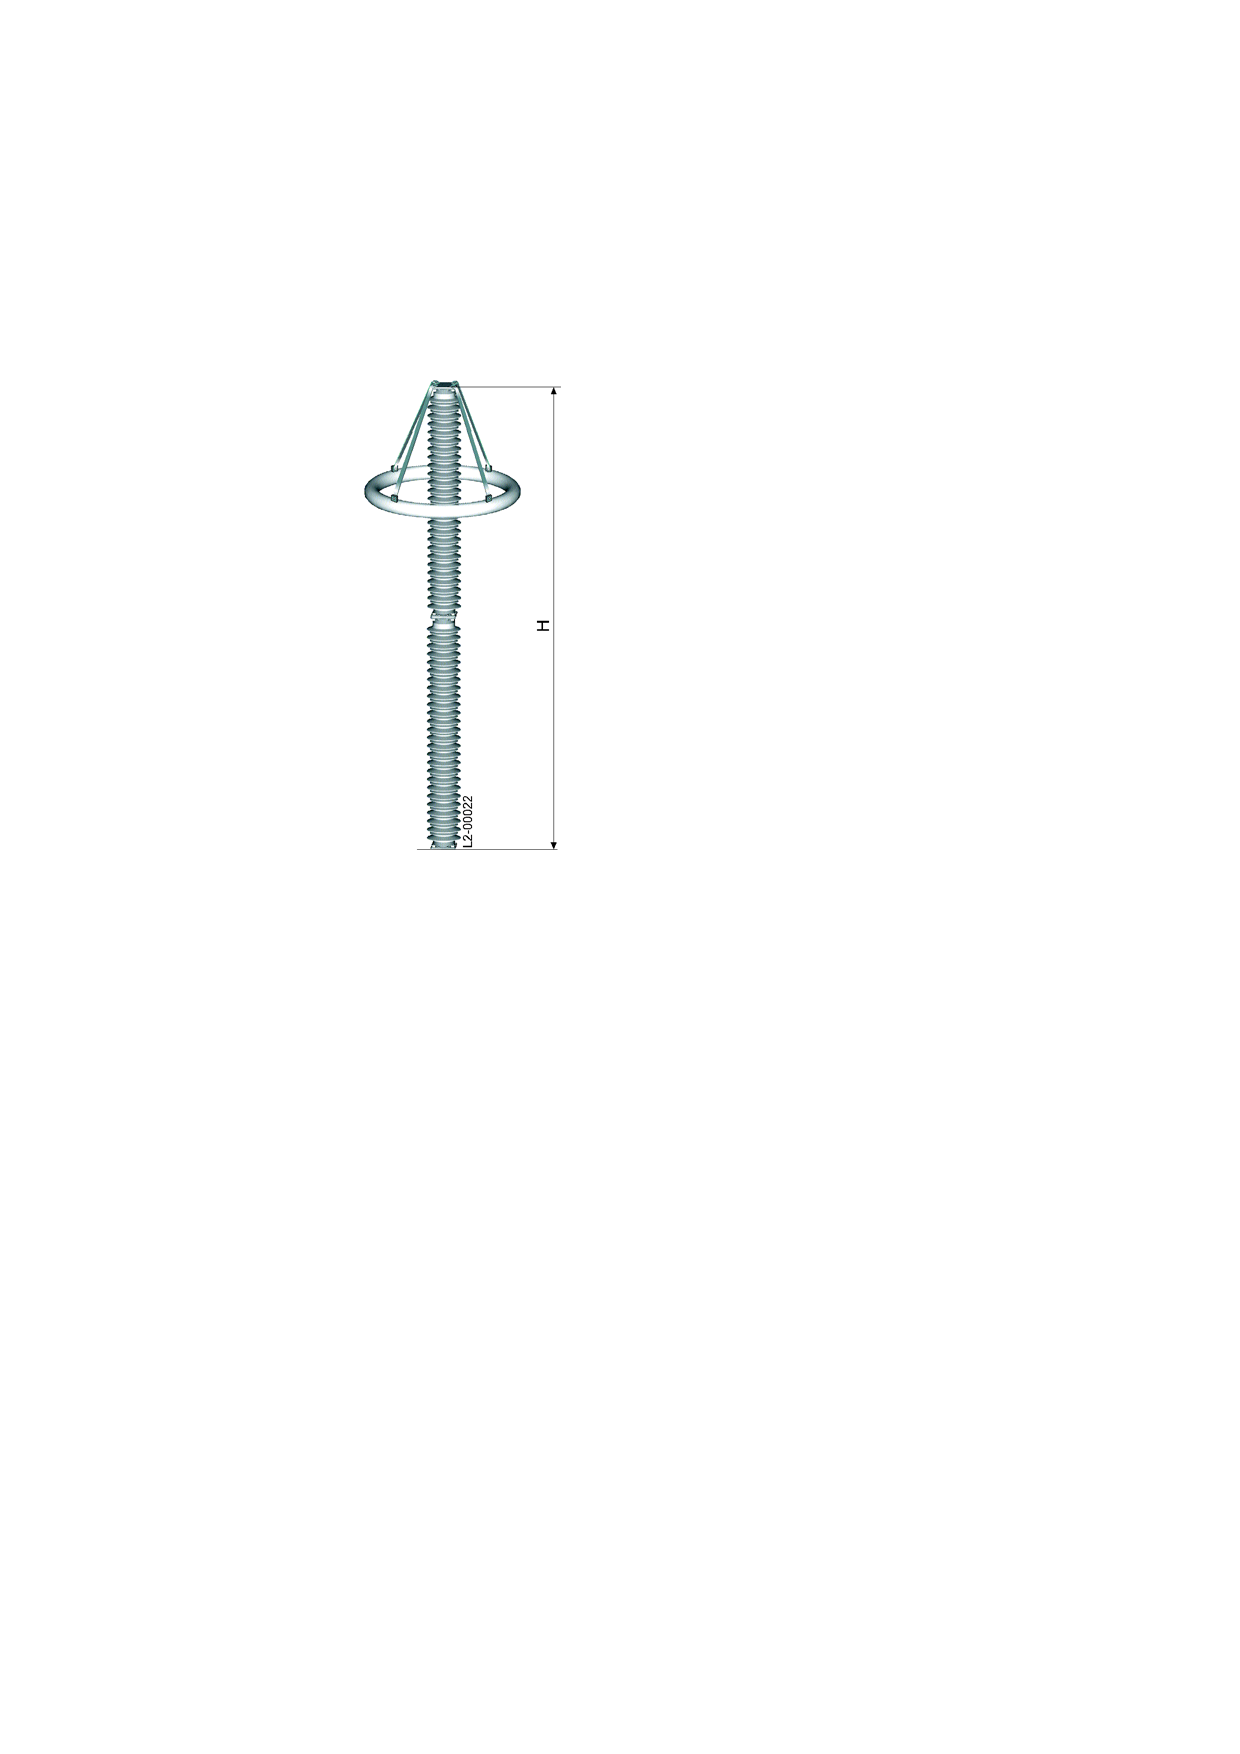
\includegraphics[width=2.7cm]{pararaio.pdf}
  \label{fig:pararaioA}
  }
  \subfloat[Placa de identificação] {
  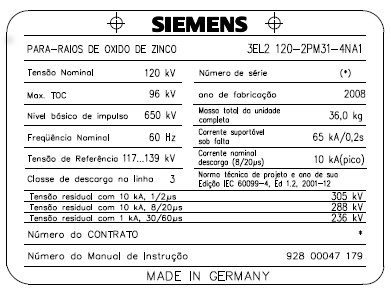
\includegraphics[width=8cm]{pararaio.jpg}
  \label{fig:pararaioB}
  }
% \legend{Fonte: Do autor}
\end{figure}

\section{Muflas e Terminações}

\section{Condutores}

\section{Transformador de Corrente (TC)}
Um transformador de corrente ou simplesmente TC é um dispositivo que reproduz no seu circuito secundário, a corrente que circula em um enrolamento primário com sua posição vetorial substancialmente mantida, em uma proporção definida, conhecida e adequada. Os transformadores de corrente, também chamados de transformadores de instrumentos, utilizados em aplicações de alta tensão (situações essas onde circulam, frequentemente, altas correntes), fornecem correntes suficientemente reduzidas e isoladas do circuito primário de forma a possibilitar o seu uso por equipamentos de medição, controle e proteção. A simbologia padrão dos transformadores de corrente mostra os terminais primários de alta tensão H1 e H2 e os terminais secundários X1 e X2, como visto na \autoref{fig:tca}.

\begin{figure}[htb]
  \caption{Simbologia e circuito equivalente simplificado do TC}
  \label{fig:tca}
  \centering
  \subfloat {
  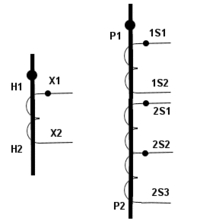
\includegraphics[width=5cm]{tca.jpg}
  }
  \subfloat {
  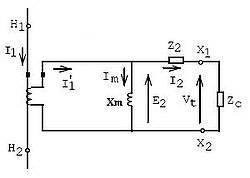
\includegraphics[width=5.8cm]{tcb.jpg}
  }
% \legend{Fonte: Do autor}
\end{figure}\par
O ponto, para transformadores com polaridade aditiva, indica onde entra a corrente no primário e onde sai a corrente no secundário (defasagem de 180º). Modelos industriais de TC’s têm os terminais de alta tensão marcados como P1 e P2 (Primário 1 e Primário 2), sendo que em muitos casos pode haver diferentes ligações do circuito primário que permitam alterar a relação de transformação. Os terminais secundários são marcados como 1s1, 1s2, 2s2 (número, algarismo, número), indicando respectivamente o número do enrolamento, o símbolo de terminal secundário (s) e o número da derivação do terminal secundário.\par
\begin{figure}[htb]
  \caption{Placa de identificação de um TC utilizado no barramento de 138 kV}
  \centering
  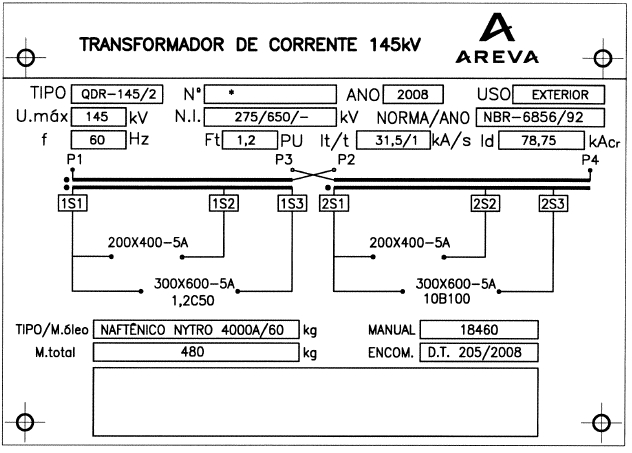
\includegraphics[width=10.8cm]{placatc.jpg}
% \legend{Fonte: Do autor}
  \label{fig:placatc}
\end{figure}

O circuito equivalente aproximado para um transformador de corrente é mostrado na Figura 10, onde a transformação da corrente entre os circuitos primário e secundário é feita sem perdas. A impedância de dispersão do primário Z1 é multiplicada pelo quadrado da relação $N^{2}$ quando referida ao secundário. A impedância de dispersão secundária é Z2. Os componentes de perdas no núcleo por correntes parasitas e por magnetização são dados por Zm e a impedância de carga é dada por Zc. Este circuito generalizado pode ser simplificado como mostrado no esquema ao lado. A impedância primária Z1 pode ser desprezada, uma vez que o reduzido número de espiras no primário (o que é verdadeiro para a maioria dos TC’s comerciais) tem pequena resistência e pouca dispersão. A corrente através do ramo magnetizante Xm é Im, chamada corrente de excitação. A corrente de excitação é atrasada de 90º em relação a V1'.\par
\begin{figure}[htb]
  \caption{Foto de um Transformador de Corrente}
  \centering
  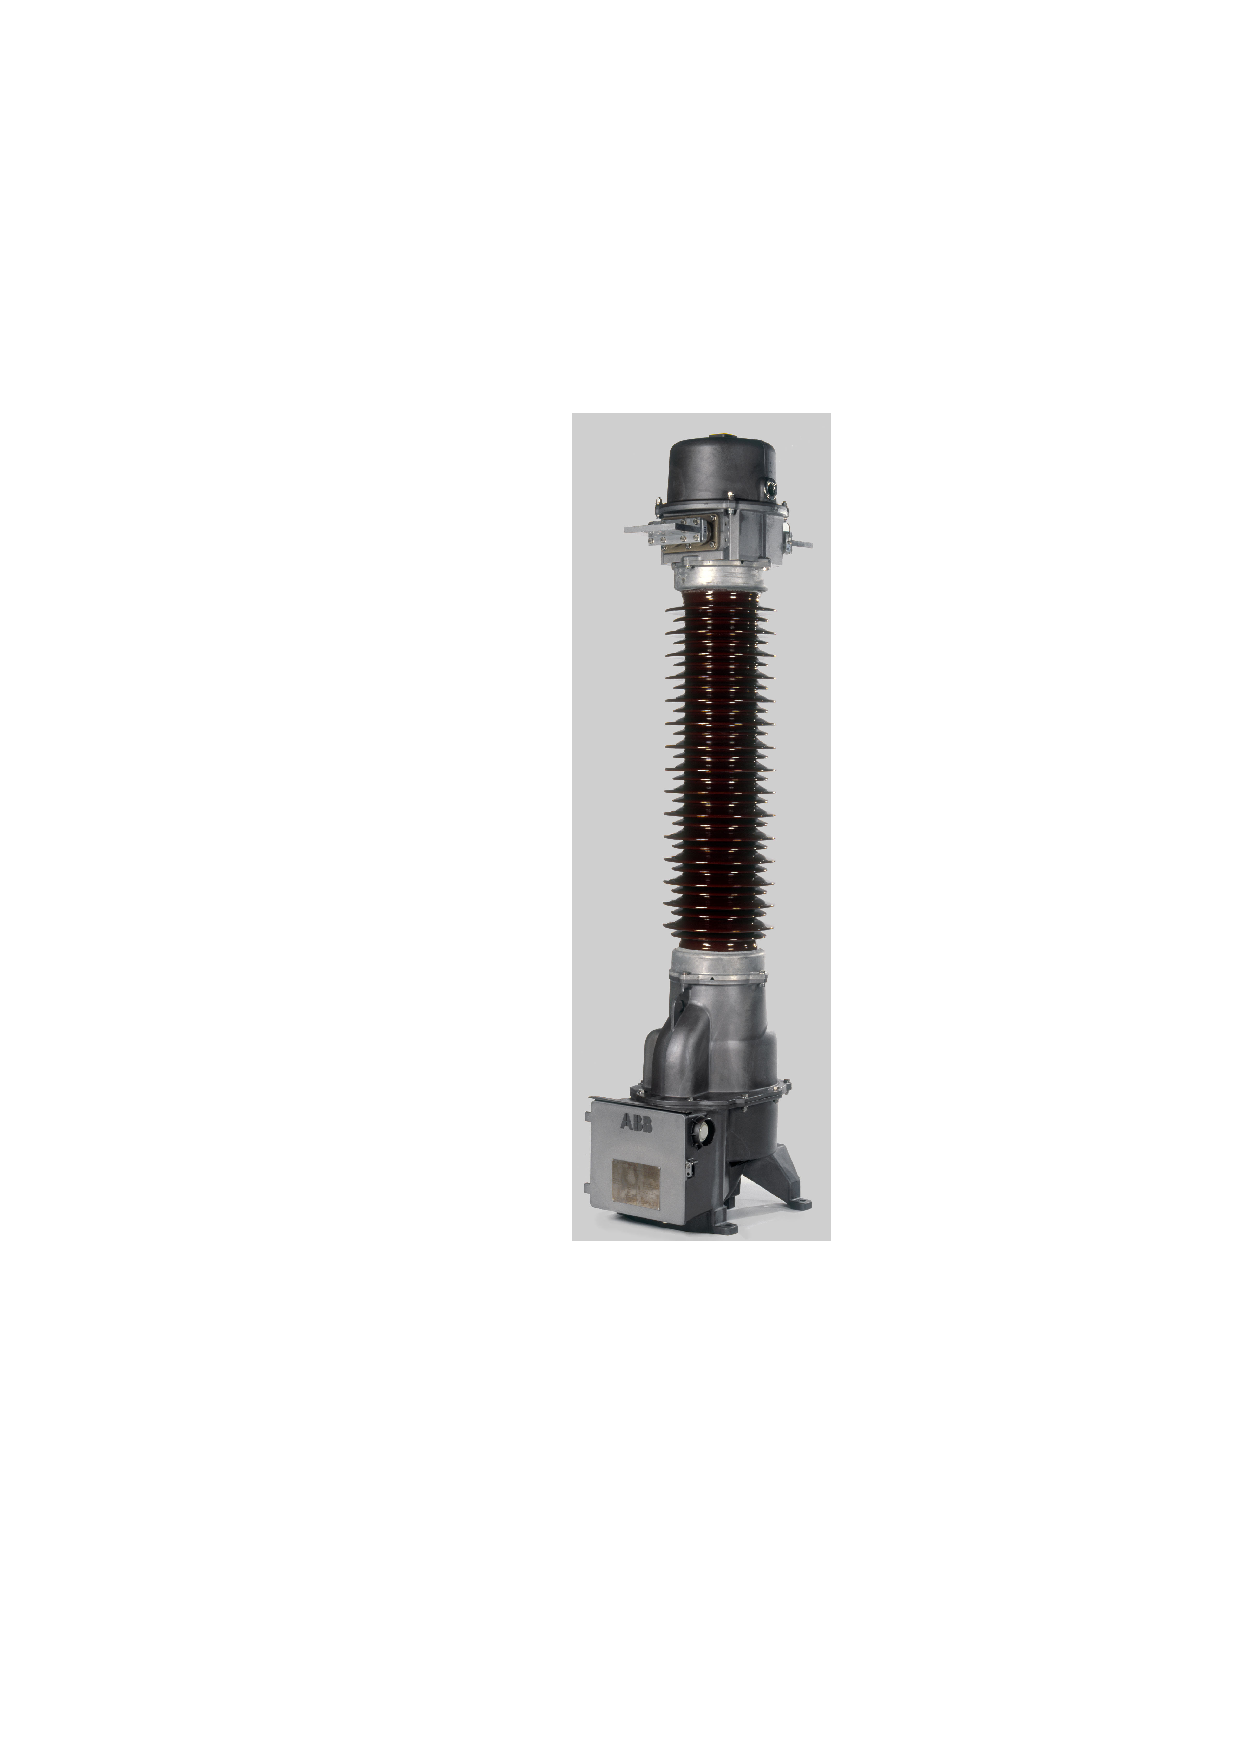
\includegraphics[width=3cm]{fototc.pdf}
% \legend{Fonte: Do autor}
  \label{fig:fototc}
\end{figure}

\section{Transformador de Potencial (TP)}
Transformador de Potencial (TP) é um equipamento usado principalmente para sistemas de medição de tensão elétrica, sendo capaz de reduzir a tensão do circuito para níveis compatíveis com a máxima suportável pelos instrumentos de medição. Sua principal aplicação é na medição de tensões com valores elevados, ou seja, em seu circuito primário é conectada a tensão a ser medida, sendo que no secundário será reproduzida uma tensão reduzida e diretamente proporcional a do primário. Assim, com menor custo e maior segurança, pode-se conectar o instrumento de medição no secundário. A razão entre a tensão no primário sobre a tensão apresentada no secundário de qualquer transformador é uma constante chamada de relação de transformação (RT). A RT é determinada na fabricação do TP pela razão entre o número de espiras do enrolamento primário sobre o número de espiras do enrolamento secundário, assim conhecendo-se a RT e a tensão no circuito secundário, tem-se o valor da tensão no circuito primário. Os TPs podem ser considerados especiais, pois são fabricados de forma a apresentar uma RT com ótima exatidão, ou seja, uma pequena variação na tensão do primário causará uma variação proporcional também no secundário, permitindo assim que indicação no instrumento de medição apresente uma incerteza de medição muito pequena. A tensão reduzida do circuito secundário do TP também é usada para alimentar, de forma igualmente segura, os circuitos de proteção e controle de subestações. Os principais componentes de um TP é mostrado na \autoref{fig:vistatp}.

\begin{figure}[htb]
  \caption{Identificação das partes de um TP}
  \centering
  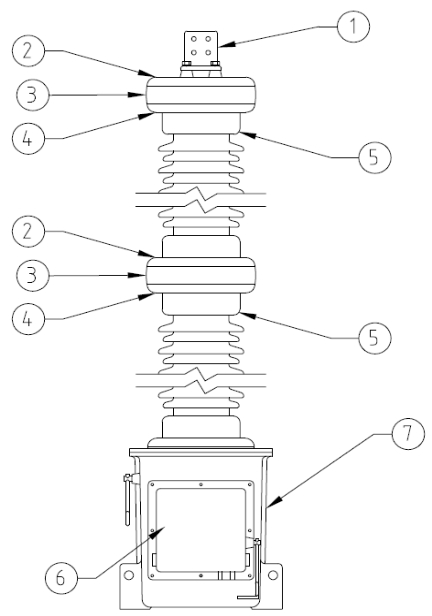
\includegraphics[width=7cm]{vistatp.jpg}
% \legend{Fonte: Do autor}
  \label{fig:vistatp}
\end{figure}

\begin{longtable}{|l|l|l|l|}
\caption{Identificação das partes de um TP}
\\ \hline
  Pos. & Componente & Material & Acabamento \\ \hline
  1 & Terminal de Linha & Liga de Alumínio & Natural \\ \hline
  2 & Placa Superior & Liga de Alumínio & A+B \\ \hline
  3 & Anel de Junção & Liga de Alumínio & A+B \\ \hline
  4 & Placa Inferior & Liga de Alumínio & A+B \\ \hline
  5 & Flange do isolador & Liga de Alumínio & A+B \\ \hline
  6 & Caixa de terminais secundários & Liga de Alumínio & A+B \\ \hline
  7 & Unidade Eletromagnética & Liga de Alumínio & A+B \\ \hline
\end{longtable}

\section{Chave seccionadora}
As chaves podem desempenhar nas subestações diversas funções, sendo a mais comum a de secionamento de circuitos por necessidade operativa, ou por necessidade de isolar componentes do sistema (equipamentos e linhas) para a realização de manutenção nos mesmos. Neste último caso, a chave aberta que isola o componente em manutenção deve ter uma suportabilidade entre terminais às solicitações dielétricas de forma que o pessoal de campo possa executar o serviço de manutenção em condições adequadas de segurança. A manutenção em uma única chave normalmente acarreta desligamentos indesejáveis nas subestações, chegando, em alguns casos, a provocar o desligamento de toda a subestação. Este caso que ocorre, por exemplo, durante a manutenção dos secionadores ligados à barra principal de subestações com arranjo barra principal/barra transferência.

\begin{figure}[htb]
  \caption{Tipos construtivos de chaves seccionadoras}
  \centering
  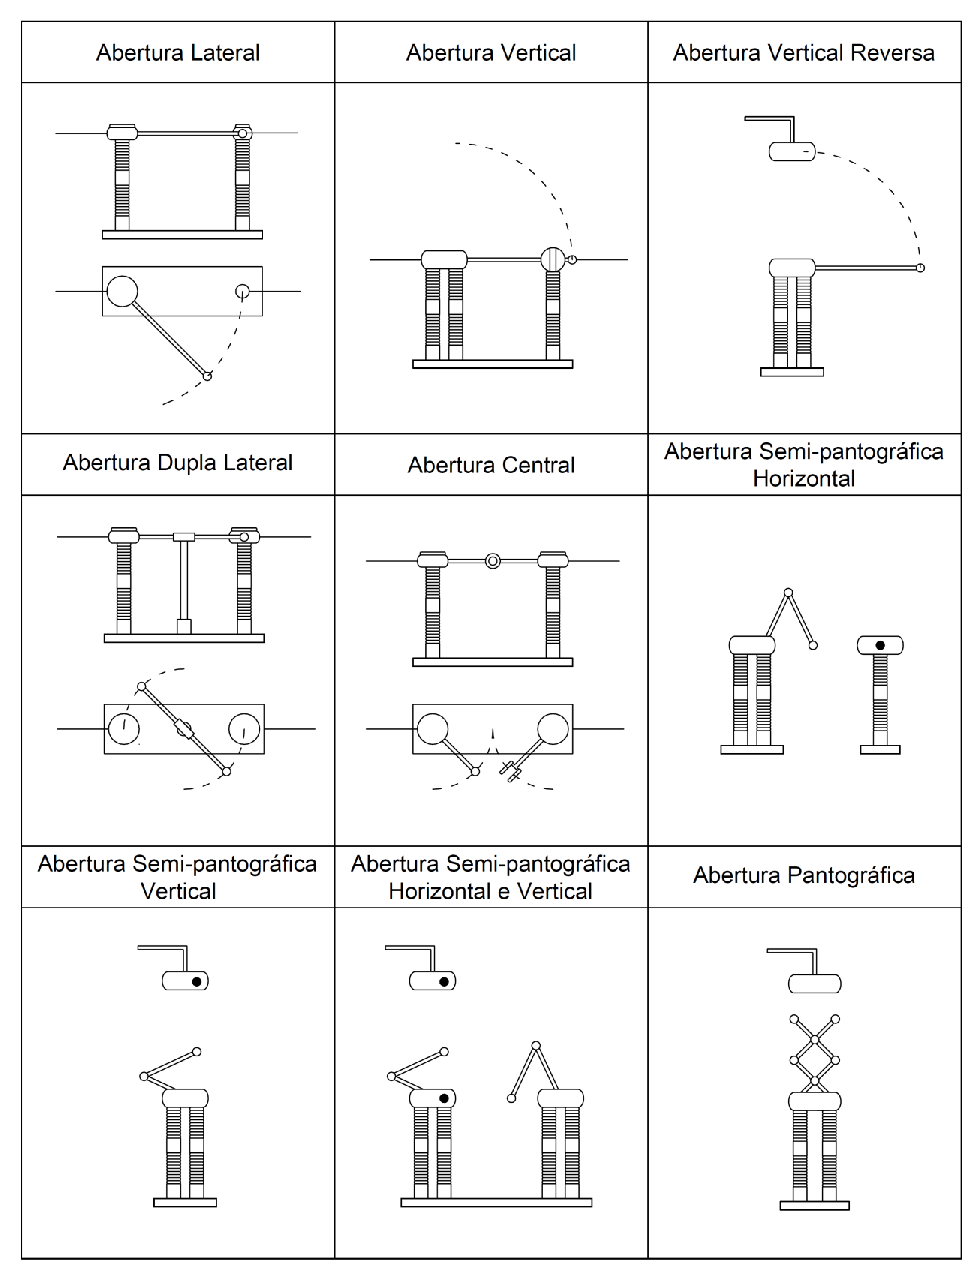
\includegraphics[width=10cm]{chavesec.pdf}
% \legend{Fonte: Do autor}
  \label{fig:chavesec}
\end{figure}

\section{Painéis}
Os quadros de baixa tensão compõem-se de um ou mais painéis modulares configurando seções verticais blindadas com dimensões padronizadas e com possibilidade de ampliar o número de módulos de um quadro através de simples acoplamento. Basicamente um painel de distribuição contém unidades de manobra de circuitos alimentadores com chave secionadora com fusíveis, ou disjuntor. A fiação de comando entre as unidades, quando houver, está disposta em canaletas verticais em cada painel e a interligação entre painéis pode ser executada no topo e/ou na parte inferior dos mesmos. Todas as unidades de controle e/ou distribuição são montadas em compartimentos individuais.

\begin{figure}[htb]
  \caption{Vistas dos painéis da casa de comando}
  \centering
  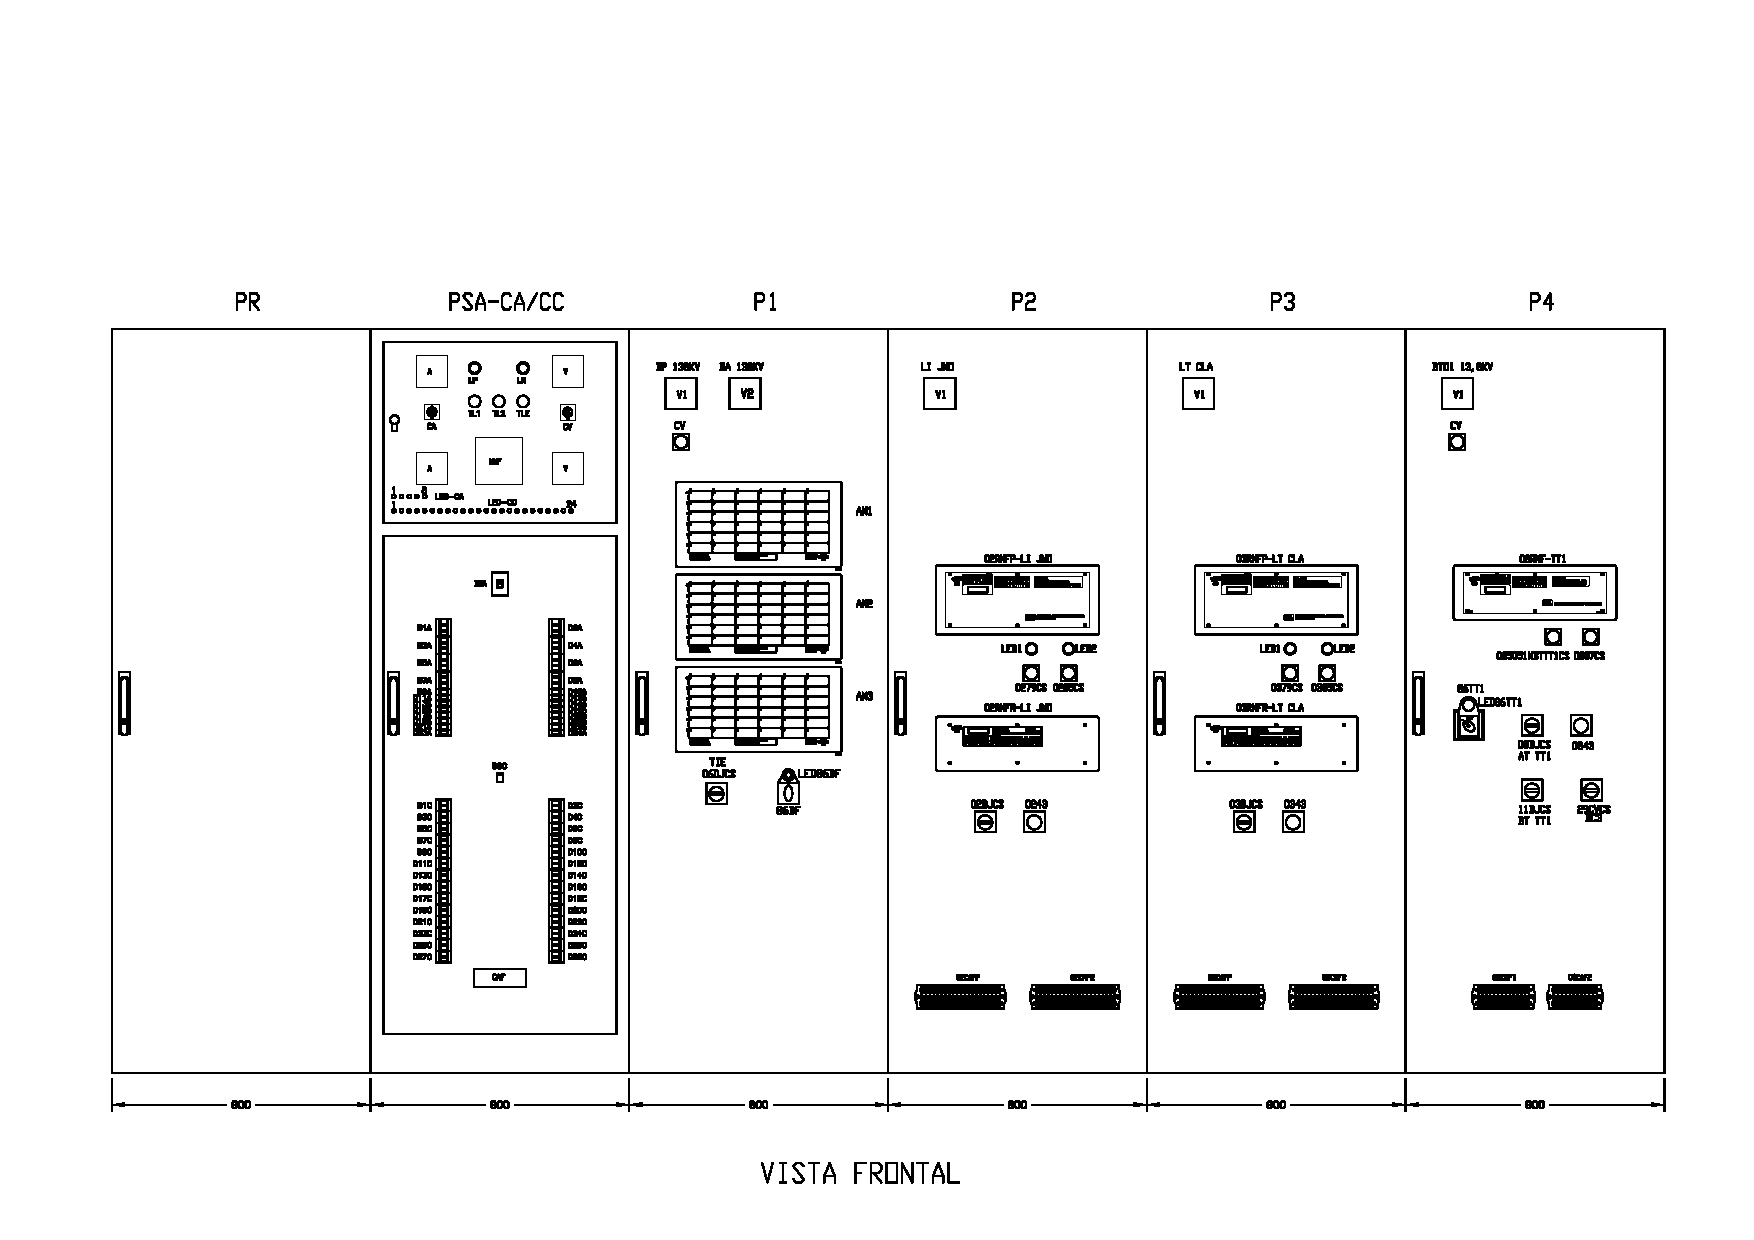
\includegraphics[width=10.8cm]{paineis.pdf}
% \legend{Fonte: Do autor}
  \label{fig:paineis}
\end{figure}

\section{Disjuntor}
Disjuntor é um dispositivo eletromecânico que permite proteger uma determinada instalação elétrica contra sobre-intensidades (curto-circuito ou sobrecarga). Sua principal característica é a capacidade de poder ser rearmado manualmente quando estes tipos de defeitos ocorrem, diferindo do fusível, que tem a mesma função, mas que fica inutilizado depois de proteger a instalação. Assim, o disjuntor interrompe a corrente em uma instalação elétrica antes que os efeitos térmicos e mecânicos desta corrente possam se tornar perigosos às próprias instalações. Por esse motivo, ele serve tanto como dispositivo de manobra como de proteção de circuitos elétricos. Atualmente é muito utilizado em instalações elétricas residenciais e comerciais o disjuntor magneto-térmico ou termomagnético, como é chamado no Brasil.\par
Esse tipo de disjuntor possui três funções:
\begin{itemize}
\item Manobra (abertura ou fecho voluntário do circuito);
\item Proteção contra curto-circuito - Essa função é desempenhada por um atuador magnético (solenóide), que efetua a abertura do disjuntor com o aumento instantâneo da corrente elétrica no circuito protegido;
\item Proteção contra sobrecarga: é realizada através de um atuador bi-metálico, sensível ao calor e provoca a abertura quando a corrente elétrica permanece, por um determinado período, acima da corrente nominal do disjuntor; 
\end{itemize}\par
As características de disparo do disjuntor são fornecidas pelos fabricantes através de duas informações principais: corrente nominal e curva de disparo. Outras características são importantes para o dimensionamento, tais como: tensão nominal, corrente máxima de interrupção do disjuntor e número de polos (unipolar, bipolar ou tri-polar).\par

\subsection{Disjuntor de alta tensão}
Para a interrupção de altas correntes, especialmente na presença de circuitos indutivos, são necessários mecanismos especiais para a interrupção do arco voltaico (ou arco elétrico), resultante na abertura dos polos. Para aplicações de grande potência, esta corrente de curto-circuito, pode alcançar valores de 100kA. Após a interrupção, o disjuntor deve isolar e resistir às tensões do sistema. Por fim, o disjuntor deve atuar quando comandado, ou seja, deve haver um alto grau de confiabilidade.\par

\begin{figure}[htb]
  \caption{Disjuntor Siemens a SF6 modelo 3AP1 FG junto a sua placa de identificação}
  \centering
  \subfloat[Disjuntor de Potência] {
  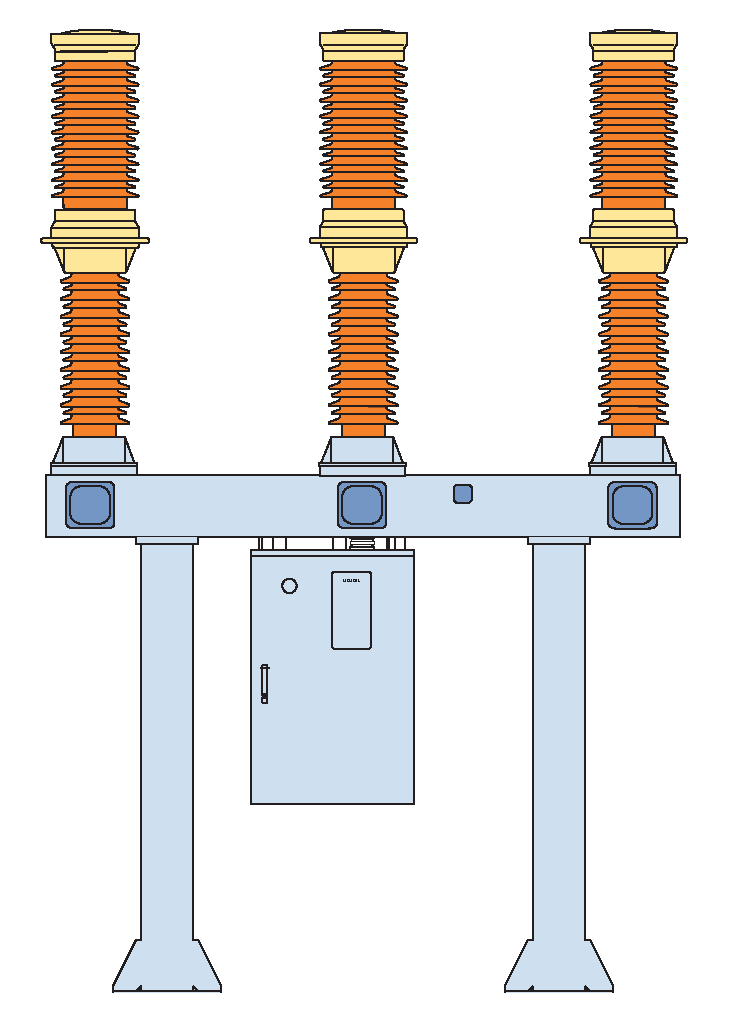
\includegraphics[width=5.5cm]{disjuntor.pdf}
  \label{fig:disjuntor}
  }
  \subfloat[Placa de identificação] {
  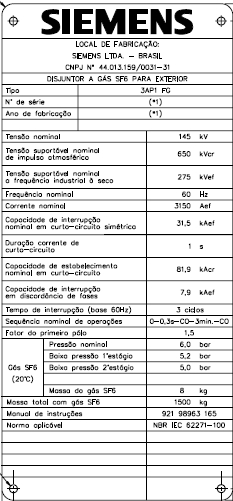
\includegraphics[width=5cm]{placadisjuntor.jpg}
  }
% \legend{Fonte: Do autor}
\end{figure}\par

Alguns tipos de disjuntores de alta potência:\par
\begin{itemize}
\item Disjuntor a grande volume de óleo;
\item Disjuntor a pequeno volume de óleo;
\item Disjuntor a ar comprimido;
\item Disjuntor a vácuo;
\item Disjuntor a hexafluoreto de enxofre (SF6); 
\end{itemize}

\section{Transformador de Potência}
A invenção do transformador de potência, que remonta o fim do século XIX, tornou-se possível o desenvolvimento do moderno sistema de alimentação em corrente alternada, com subestações de potência freqüentemente localizadas a muitos quilômetros dos centros de consumo (carga). Antes disto, nos primórdios do suprimento de eletricidade pública, estes eram sistemas de corrente contínua, com a fonte de geração, por necessidade, localizados próximo do local de consumo.\par
Indústrias pioneiras no fornecimento de eletricidade foram rápidas em reconhecer os benefícios de uma ferramenta a qual poderia dispor alta corrente, normalmente obtida a baixa tensão de saída de um gerador elétrico, e transformá-lo para um determinado nível de tensão possível de transmiti-la em condutores de dimensões práticos a consumidores que, naquele tempo, poderiam estar afastados a um quilômetro ou mais e poderiam fazer isto com uma eficiência e que, para os padrões da época, era nada menos que fenomenal.\par
Um sistema de corrente alternada opera, em cada uma de suas partes, com a tensão mais conveniente, tanto do ponto de vista técnico quanto do ponto de vista econômico. Assim, têm-se tensões entre 13,8 e 25 kV na geração, entre 138 e 765 kV na transmissão, entre 13,8 e 34,5 kV na distribuição. Esta enorme flexibilidade é obtida através dos transformadores, equipamentos estáticos, de alta eficiência e grande confiabilidade. O princípio de funcionamento é ilustrado na Figura . Sobre circuito magnético, formado de chapas de aço-silício, enrolam-se duas bobinas com N1 e N2 espiras, respectivamente. Supondo-se que o fluxo alternado $\phi$ circule, apenas, no circuito magnético, e desprezando-se as resistências, tensão por espira será constante e V1/V2=N2/N1. Estas simples relações, bastante próximas das verificadas na prática, mostram como é possível transformar tensões e correntes e interligar, assim diferentes partes de um sistema de transmissão.

\begin{figure}[htb]
  \caption{Princípio básico de um transformador}
  \centering
  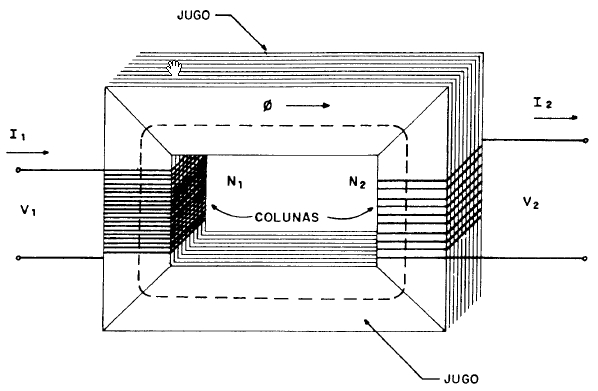
\includegraphics[width=10.8cm]{transformador.jpg}
% \legend{Fonte: Do autor}
  \label{fig:transformador}
\end{figure}

Os transformadores elevadores de usinas são de dois enrolamentos, o primário em delta e o secundário em estrela aterrada. Os demais transformadores do sistema são, em geral, autotransformadores, em estrela aterrada. Os autotransformadores, geralmente, possuem enrolamento terciário em delta, de 13,8 kV, para ligação de compensação reativa e/ou para alimentação de serviços auxiliares, com 1/3 da potência dos outros enrolamentos. Quando o terciário não for necessário para essas funções, sua exclusão depende de estudos de circulação de harmônicos de seqüência zero, de estudos de energização e de sua necessidade ou não para a realização de ensaios.\par

\begin{figure}[htb]
  \caption{Tipos de enrolamentos de transformadores de potência}
  \centering
  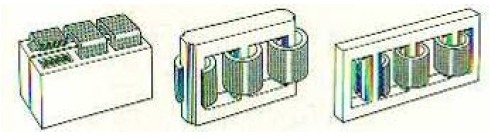
\includegraphics[width=10.8cm]{tiposdetrafo.jpg}
% \legend{Fonte: Do autor}
  \label{fig:tiposdetrafo}
\end{figure}

\begin{figure}[htb]
  \caption{Tipos de ligação dos enrolamentos de um transformador de potência}
  \centering
  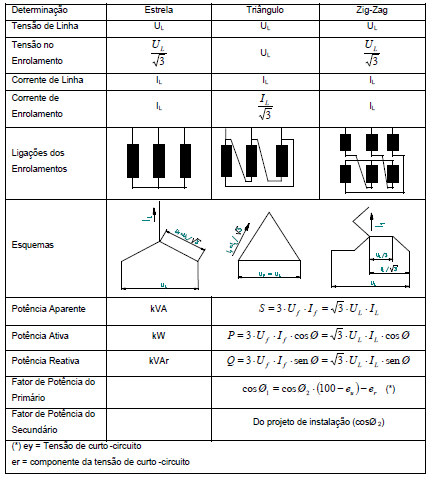
\includegraphics[width=10.8cm]{tiposdenrol.jpg}
% \legend{Fonte: Do autor}
  \label{fig:tiposdenrol}
\end{figure}

\begin{figure}[htb]
  \caption{Placa de identificação de um transformador de potência}
  \centering
  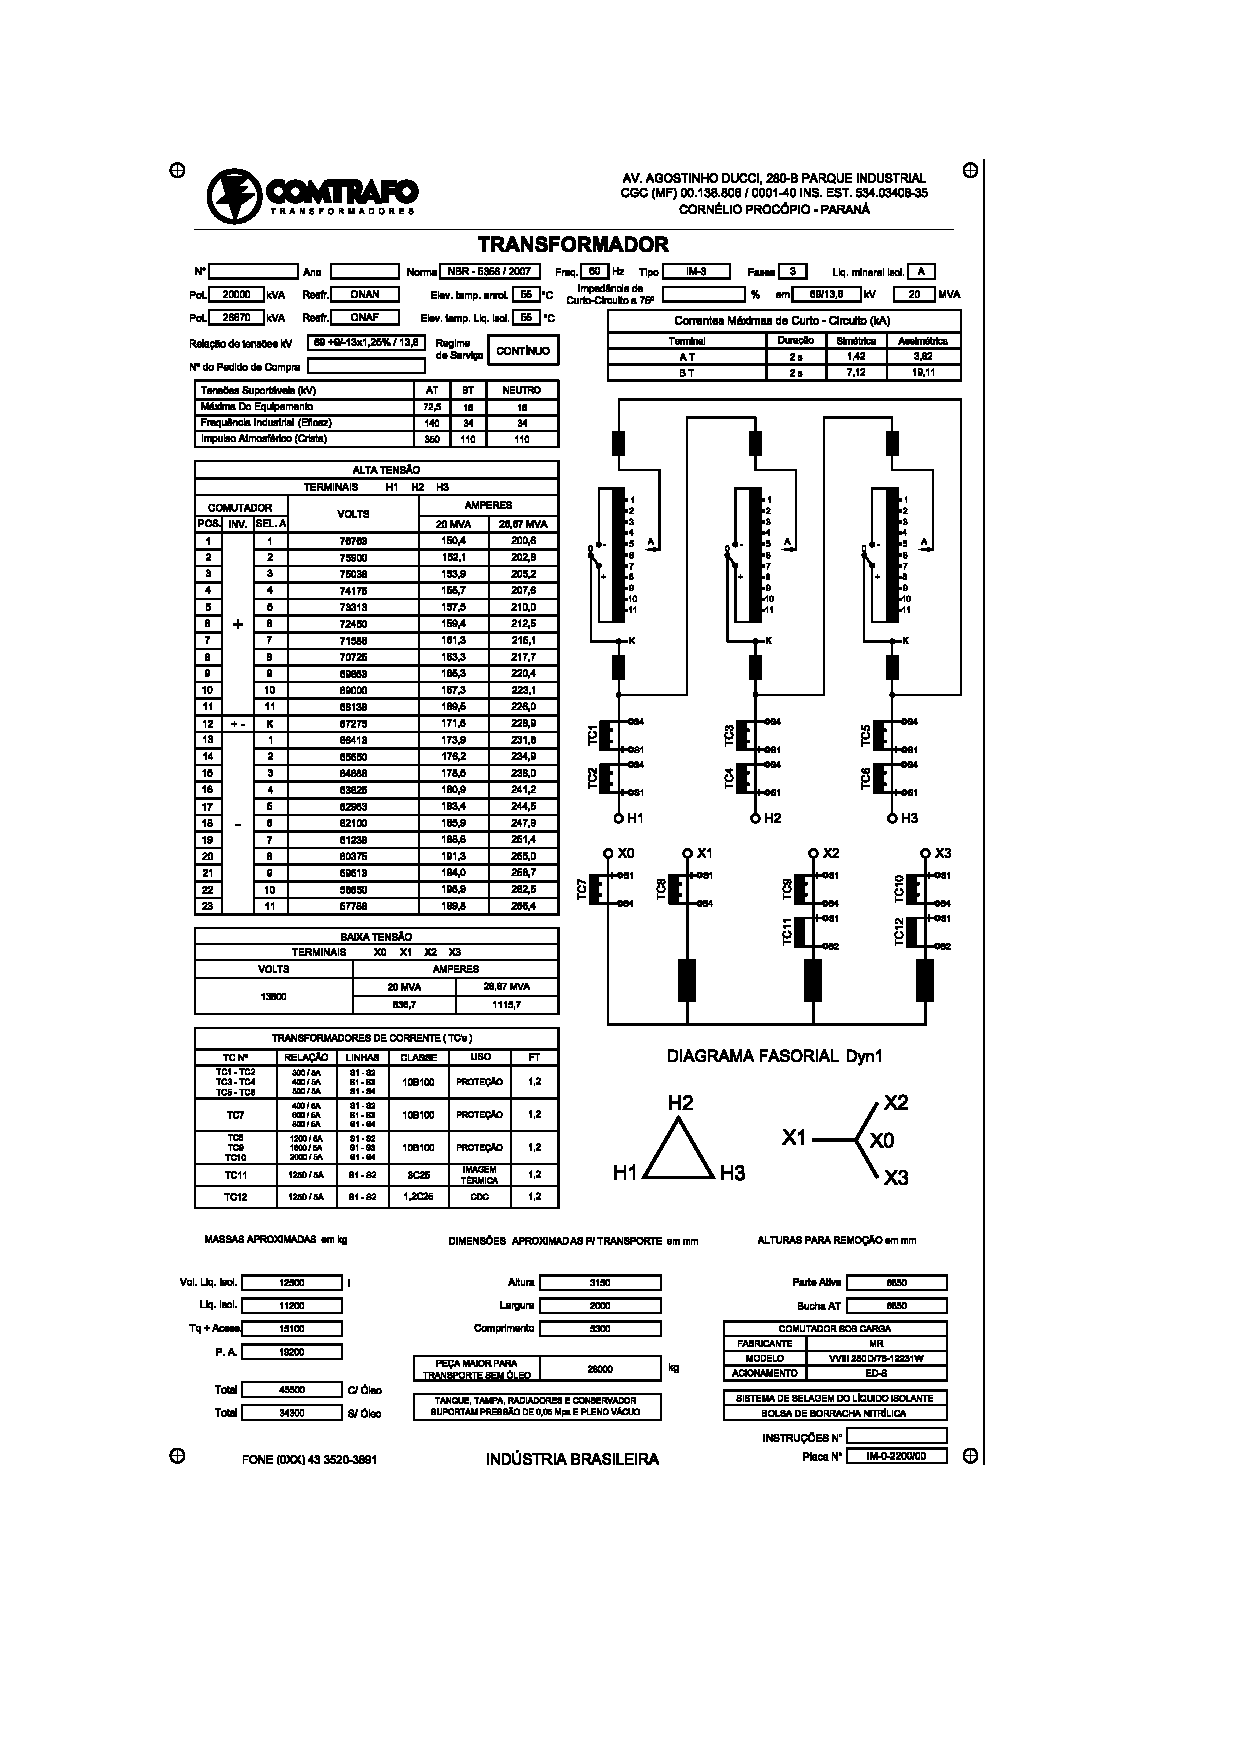
\includegraphics[width=10.8cm]{placatrafo.pdf}
% \legend{Fonte: Do autor}
  \label{fig:placatrafo}
\end{figure}

\subsection{Derivações}
Para adequar a tensão primária do transformador à tensão de alimentação, o enrolamento primário, normalmente TS, é dotado de derivações (TAPs), que podem ser escolhidos mediante a utilização de um painel de ligações ou comutador, conforme projeto e tipo construtivo, instalados junto à parte ativa, dentro do tanque. Este aparato, na maioria dos transformadores de potência, deve ser manobrado com o transformador desconectado da rede de alimentação.

\subsection{Acessórios}
Outros componentes são necessários para o perfeito funcionamento do
transformador. Na tabela 5 encontra-se este componentes chamados acessórios, em
função da potência. São os acessórios que informam através de seus contatos, as
condições de operação do transformador.

\subsubsection{Indicador de Nível de Óleo}
O óleo isolante do transformador se dilata ou se contrai conforme a variação da temperatura ambiente e variação da carga alimentada pelo transformador, em função disso, haverá elevação ou abaixamento no nível de óleo. Sendo assim, a finalidade do indicador de nível de óleo é mostrar com perfeição o nível de óleo no visor e ainda servir como aparelho de proteção ao transformador. O ponteiro indicador de nível de óleo é movimentado por meio de dois magnéticos (ímãs) permanentes, que são acoplados a um flutuador (bóia). O movimento é efetuado pela bóia, de acordo com o nível de óleo, que transmite indicações precisas ao ponteiro, devido a grande sensibilidade dos magnéticos.

\subsubsection{Temômetro de Óleo}
O termômetro é utilizado para indicação da temperatura do óleo, e o termômetro conhecido como termômetro com capilar é usado em transformadores de potência. São constituídos de um bulbo, um capilar e um mostrador, o mostrador é constituído de uma caixa, um visor com indicador, micro-ruptores, dois a quatro ponteiros de limite, que se movimentam apenas por ação externa, e um ponteiro d e indicação de temperatura máxima. Este ponteiro é impulsionado pela agulha de temperatura, apenas quando em ascensão desta, pois na redução fica imóvel, possibilitando assim, a verificação da temperatura máxima atingida em um dado período. Conforme a variação da temperatura do bulbo, o líquido (fluído térmico) em seu interior sofre dilatação ou contração, transmitindo a variação de temperatura até o mecanismo interno do mostrador do termômetro, no mesmo instante o ponteiro indicador é acionado. Quando o valor da temperatura atingir os valores ajustados para fechamento dos micro-ruptores, o sinal será transmitido ao sistema de proteção podendo acionar o alarme, desligando e fazendo o controle automático do dispositivo de resfriamento do transformador imerso em óleo.

\subsubsection{Transformador de Corrente}
São utilizados para obter a corrente de qualquer dos enrolamentos do transformador. Os transformadores de corrente tipo bucha, são constituídos apenas do enrolamento secundário pois o primário é obtido diretamente do cabo de conexão entre a bucha e o enrolamento do transformador no qual o TC está instalado e podem ser de medição ou de proteção.

\subsubsection{Termômetro do Enrolamento com Imagem Térmica}
A imagem térmica é a técnica utilizada para medir a temperatura no enrolamento do transformador. Ela é denominada imagem térmica por reproduzir indiretamente a temperatura do enrolamento. A temperatura do enrolamento, que é a parte mais quente do transformador, é a temperatura do óleo acrescida da sobre-elevação da temperatura do enrolamento em relação ao óleo. O termômetro do enrolamento com imagem térmica e seu diagrama esquemático é composto de uma resistência de aquecimento e um sensor de temperatura simples ou duplo, ambos encapsulados e montados em um poço protetor, imerso em uma câmara de óleo. O conjunto é instalado na tampa do transformador, equalizando-se com a temperatura do topo do óleo. A resistência de aquecimento é alimentada por um transformador de corrente associado ao enrolamento (normalmente) secundário do transformador principal indicando assim a temperatura no ponto mais quente do enrolamento. Portanto, a elevação da temperatura da resistência de aquecimento é proporcional à elevação da temperatura do enrolamento além da temperatura máxima do óleo. A constante do tempo do sistema é da mesma ordem de grandeza do enrolamento, logo o sistema reproduz uma verdadeira imagem térmica da temperatura do enrolamento.

\subsubsection{Controladores Micro-Processados de Temperatura}
Os controladores micro-processados de temperatura e nível de óleo foram desenvolvidos para substituir, com vantagens da tecnologia micro-processada, os termômetros de óleo e enrolamento e indicadores de nível tradicionais utilizados em transformadores e reatores de potência. Este equipamento recebe o valor da resistência de um sensor e o transforma (através de um transdutor incorporado) em temperatura equivalente, a qual é vista em painel frontal digital, podendo ser transmitida remotamente através de interface serial RS485 ou sinal analógico. Desempenha diversas funções de controle e acionamento de contatos, sendo que através de teclado frontal podemos configurar os parâmetros de sua atuação e ler os valores medidos e ajustados.

\subsubsection{Válvula de Alívio de Pressão}
A válvula de alívio de pressão, de fechamento automático, instalada em transformadores imersos em líquido isolante, tem a finalidade de protegê-los contra uma possível deformação ou ruptura do tanque em casos de defeitos internos com aparecimento de pressão elevada. A válvula é extremamente sensível e rápida (opera em menos de dois milésimos de segundo), fecha-se automaticamente após a operação impedindo assim a entrada de qualquer agente externo no interior do transformador. Possui contatos para alarme e desligamento.

\subsubsection{Relê Detector de Gás Tipo Buchholz}
O relé de gás tem por finalidade proteger equipamentos imersos em líquido isolante, através da supervisão do fluxo anormal do óleo ou ausência, e a formação anormal de gases pelo equipamento. São utilizados em transformadores que possuem tanque para expansão de líquido isolante. Este tipo de relé detecta de forma precisa, por exemplo, os seguintes problemas: vazamento de líquido isolante, curto-circuito interno do equipamento ocasionando grande deslocamento de líquido isolante, formação de gases internos devido a falhas intermitentes ou contínuas que estejam ocorrendo no interior do equipamento. O relé detector de gás é normalmente instalado entre o tanque principal e o tanque de expansão do óleo dos transformadores. A carcaça do relé é de ferro fundido, possuindo duas aberturas flangeadas e ainda dois visores nos quais está indicada uma escala graduada de volume de gás. Internamente encontram-se duas bóias de gás no relé, a bóia superior é forçada a descer em caso de acúmulo de gás (isto acontece também caso haja vazamento de óleo). Se por sua vez uma produção excessiva de gás provoca uma circulação de óleo no relé, é a bóia inferior que reage, antes mesmo que os gases formados atinjam o relé. Em ambos os casos, as bóias ao sofrerem o deslocamento acionam contatos.

\subsubsection{Secador de Ar de Sílica Gel}
O secador de ar de sílica gel é usado nos transformadores providos de conservador de óleo, funcionando como um desumidificador de ar do transformador. Para evitar a deterioração do óleo do equipamento ou bolsa de borracha pelas impurezas e umidade no ar respirado, coloca-se um copo com óleo e sílica gel na passagem por onde o ar é suspirado. Quando o nível do óleo no conservador baixar, haverá o respiro de ar atmosférico, este ar passará primeiramente pelo copo de óleo, onde ficarão eliminadas as impurezas sólidas e em seguida o ar atravessa os cristais de sílica gel, que retiram a umidade do ar, em seguida, já totalmente limpo e sem umidade, o ar penetra no conservador. O ar ao passar pela sílica gel deixará na mesma a umidade, fazendo que a sílica gel troque de coloração, até a sua saturação conforme indicado abaixo:\par
\begin{itemize}
\item coloração laranja: sílica gel seca;
\item coloração amarela: sílica gel com aproximadamente 20\% da umidade absorvida;
\item  coloração amarelo-claro: sílica gel com 100\% de umidade absorvida (saturada); para regeneração da sílica gel recomenda-se colocar em estufa com temperatura máxima de 120ºC de 2 a 4 horas. 
\end{itemize}

\subsubsection{Relé de Pressão Súbita}
O relê de pressão súbita é um equipamento de proteção para transformadores do tipo selado. Normalmente o relé de pressão súbita é instalado acima do nível máximo do líquido isolante, no espaço compreendido entre o líquido isolante e a tampa do transformador. Entretanto é aceitável também a montagem horizontal, sobre a tampa do transformador. O relé é projetado para atuar quando ocorrem defeitos no transformador que produzem pressão interna anormal, sendo sua operação ocasionada somente pelas mudanças rápidas da pressão interna independente da pressão de operação do transformador. Por outro lado, o relé não opera devido a mudanças lentas de pressão, próprias do funcionamento normal do transformador, bem como durante perturbações do sistema (raios, sobre-tensão de manobra ou curto-circuito), a menos que tais perturbações produzam danos no transformador.

\subsubsection{Manômetro e Manovacuômetro}
O manômetro é um instrumento utilizado para medir a pressão interna do tanque de óleo. E o manovacuômetro mede pressão e vácuo. Podem possuir contatos de atuação.

\subsubsection{Indicador de Fluxo de Óleo}
O indicador de fluxo indica a vazão em circuitos de resfriamento de transformadores. O princípio de funcionamento é um sistema de palheta fixa a um eixo transversal, fazendo girar uma haste e cujo movimento é regulado por uma mola. O movimento do eixo ao ponteiro é transmitido por imãs permanentes, acoplados magneticamente, através de uma parede que isola a parte inferior do tubo ao lado externo. O mecanismo externo de indicação aloja também o(s) contato(s) elétrico(s).O acionamento sinaliza a ausência de fluxo, sendo necessário uma vazão nominal conforme tabela 8.

\subsubsection{Relé Regulador de Tensão}
Tem como finalidade manter a tensão do transformador sob a mesma tensão da rede de alimentação. Através de um transformador de potencial e um transformador de corrente instalados na rede de alimentação (normalmente no lado de baixa tensão), faz um comparativo entre a tensão na rede e o valor nele ajustado da tensão e corrente nominais a serem fornecidas. Caso os valores permanecerem divergentes por tempo maior do que um pré-ajustado, o equipamento, através do fechamento de seus contatos envia sinais de “elevar TAP” ou “baixar TAP” ao mecanismo motorizado do comutador sob carga. Também possuem proteção contra sobre-corrente, sub-tensão e sobre-tensão, bloqueando a comutação sob carga em caso de ocorrência.

\subsubsection{Paralelismo entre Transformadores}
Respeitadas as condições de rede de paralelismo entre os transformadores, o comando dos circuitos auxiliares pode ser colocado para trabalhar em paralelo da seguinte maneira: o controle pode ser feito por um sistema analógico, através de lógica com contatos ou pode também ser feito com sistema micro-processado. O sistema micro-processado reduz consideravelmente as dimensões da caixa de equipamentos auxiliares, possibilita o controle e supervisão (local e remota) da operação em paralelo de transformadores equipados com comutadores de derivação em carga. O sistema feito através da lógica de contatos também poderá ter indicação remota, porém será necessária a utilização de diversos componentes elétricos e eletrônicos para desempenhar todas as funções feitas com apenas dois equipamentos micro-processados. Modelos atuais de relés reguladores de tensão incluem saídas para utilização em paralelo com demais relés reguladores. Desta forma pode-se trabalhar com até 6 transformadores em paralelo, sendo necessário para tal, que cada transformador possua seu equipamento. Quando o paralelismo é feito através de equipamento específico, é necessário apenas um relé regulador de tensão para cada transformador, porém é necessário um equipamento de paralelismo para cada transformador.\par
Existem dois métodos para o paralelismo de transformadores com CDC:\par
\begin{itemize}
\item Corrente circulante: o objetivo deste sistema é manter a corrente de circulação entre os transformadores a menor possível, admitindo assim pequena diferença nos TAP do comutador;
\item Mestre-comandado (padrão da NBR 9368): os controladores quando colocados em paralelo com os transformadores no mesmo TAP, o mantém durante as comutações, transmitindo o comando do primeiro transformador (mestre) para os demais (comandados). Não admite diferença de TAP entre os transformadores.
\end{itemize}
O diagrama esquemático de comutação sob carga com relé regulador de tensão e supervisor de paralelismo com sistema micro-processado é mostrado na figura 31.\par

\subsubsection{Monitoramento de Buchas}
O monitor de buchas permite que seja efetuada de forma \textit{on-line}, durante a operação normal, a monitoração da capacitância e do fator de dissipação da isolação de buchas, TC’s e outros equipamentos. Com isso, podem ser evitadas falhas potencialmente catastróficas, ao se detectar os problemas ainda em fase incipiente. A forma construtiva da bucha capacitiva dá origem a uma capacitância entre o condutor central da bucha e o terra. Uma vez energizada a bucha, esta capacitância permite a passagem de uma corrente de fuga para o terra. Esta corrente também possui componente resistiva. Qualquer alteração nestes dois parâmetros da isolação da bucha causa uma mudança correspondente na corrente de fuga. Opera medindo continuamente as correntes de fuga das 3 buchas de um conjunto trifásico, através de adaptadores conectados aos TAPs de teste ou TAPs de tensão de cada bucha e compara estes valores com os valores iniciais das buchas obtidos em ensaios do fabricante, no caso de buchas novas, ou de ensaios off-line realizados na instalação do Monitor de Buchas. É composto pelo adaptador (1 por bucha), módulo de medição (1 para cada 3 buchas do enrolamento de mesmo nível de tensão) e módulo de interface (1 para até 3 níveis de tensão do mesmo transformador).

\subsubsection{Monitor de Gás e Umidade}
Os gases combustíveis dissolvidos no óleo de equipamentos de Alta Tensão são reconhecidamente um dos melhores indicadores do estado interno do equipamento e de sua isolação, e o hidrogênio é considerado um gás chave por estar presente na maioria dos defeitos em transformadores, podendo indicar a ocorrência de falhas ainda em fase incipiente. O Monitor de Gás e Umidade “GMM” efetua a monitoração on-line da quantidade de hidrogênio dissolvido em óleo mineral isolante, emitindo alarmes tanto por níveis de hidrogênio acima do limite estabelecido, quanto por taxa de aumento elevada. Mede o conteúdo de hidrogênio sem interferência cruzada de outros gases, como por exemplo, o CO. Desta forma é obtida a máxima sensibilidade na detecção de defeitos, sem que as alterações no hidrogênio sejam encobertas por concentrações constantes e muitas vezes mais elevadas de CO. O GMM monitora também a saturação de água no óleo (0 a 100\%) e a temperatura do óleo associada, calculando o teor de água (ppm) no óleo isolante. O Monitor de Gás e Umidade é composto pelo Módulo de Medição e pelo Módulo de Interface. O Módulo de Medição deve ser acoplado a uma válvula de óleo do tipo passagem livre localizada em local com boa circulação de óleo. Possui uma porta de comunicação serial RS485, através da qual são transmitidas as informações ao Módulo de Interface, que disponibiliza as informações localmente em seus displays e remotamente através das saídas analógicas, saídas a contatos secos e pelas portas seriais RS485 e RS232 com protocolos Modbus RTU e DNP3.0. O Módulo de Interface efetua também os cálculos de tendência e o armazenamento de valores históricos em memória não volátil.

\section{Relés}
Os relés são os elementos mais importantes dos sistemas de proteção. A função primordial deles é identificar os defeitos, localizá-los da maneira mais exata possível e alertar a quem opera o sistema; promovendo o disparo de alarmes, sinalizações e enviando sinais para a abertura de disjuntores de modo a isolar o defeito.\par

\subsection{Relé de Sobrecorrente}
São todos os relés que atuam para uma corrente maior que a do seu ajuste. Caso ocorra uma falha no sistema e a corrente de curto-circuito ultrapassar a corrente de ajuste do sensor do relé, o mesmo atua instantaneamente ou temporizado, conforme a necessidade.\par

\subsection{Relé Eletromecânico}
São os relés pioneiros da proteção, projetados e construídos com predominância dos movimentos mecânicos provenientes dos acoplamentos elétricos e magnéticos. Quando o relé de sobre-corrente eletromecânico opera, fecha o seu contato, energizando o circuito DC que irá comandar a operação de abertura do disjuntor.\par

\begin{figure}[htb]
  \caption{Especificação de um relé eletromecânico da marca Finder}
  \centering
  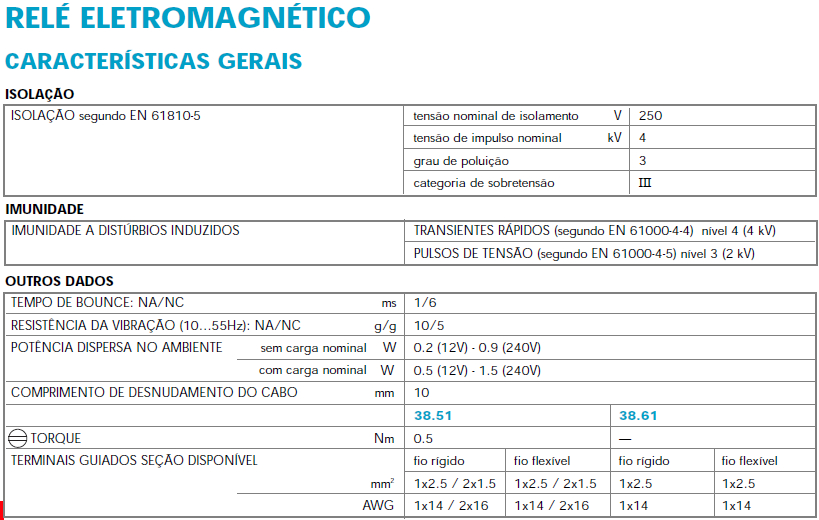
\includegraphics[width=10.8cm]{eletromag.jpg}
% \legend{Fonte: Do autor}
  \label{fig:eletromag}
\end{figure}

\subsection{Relé de indução eletromagnética}
Este relé, também conhecido como relé motorizado, funciona utilizando o mesmo princípio de um motor de indução, onde um rotor (tambor ou disco) gira. O giro do rotor produz o fechamento do contato NA do relé, que ativa o circuito ou mecanismo que provoca a abertura do disjuntor.\par

\subsection{Relé eletrônico ou estáticos}
São relés construídos com dispositivos eletrônicos, próprios e específicos aos objetivos da proteção. Nestes relés, não há nenhum dispositivo mecânico em movimento, todos os comandos e operações são feitos eletronicamente.\par

\subsection{Relé digital}
São relés eletrônicos gerenciados por microprocessadores específicos a este fim, onde sinais de entrada das grandezas e parâmetros digitados são controlados por \textit{software} que processa a lógica da proteção através de algoritmos. O relé digital pode simular um relé ou todos os relés existentes em um só equipamento, produzindo ainda outras funções, tais como, medições de suas grandezas de entradas e/ou associadas, sendo conhecido como relé multi-função.\par

\begin{figure}[htb]
  \caption{Relé SEL-351A para linhas}
  \centering
  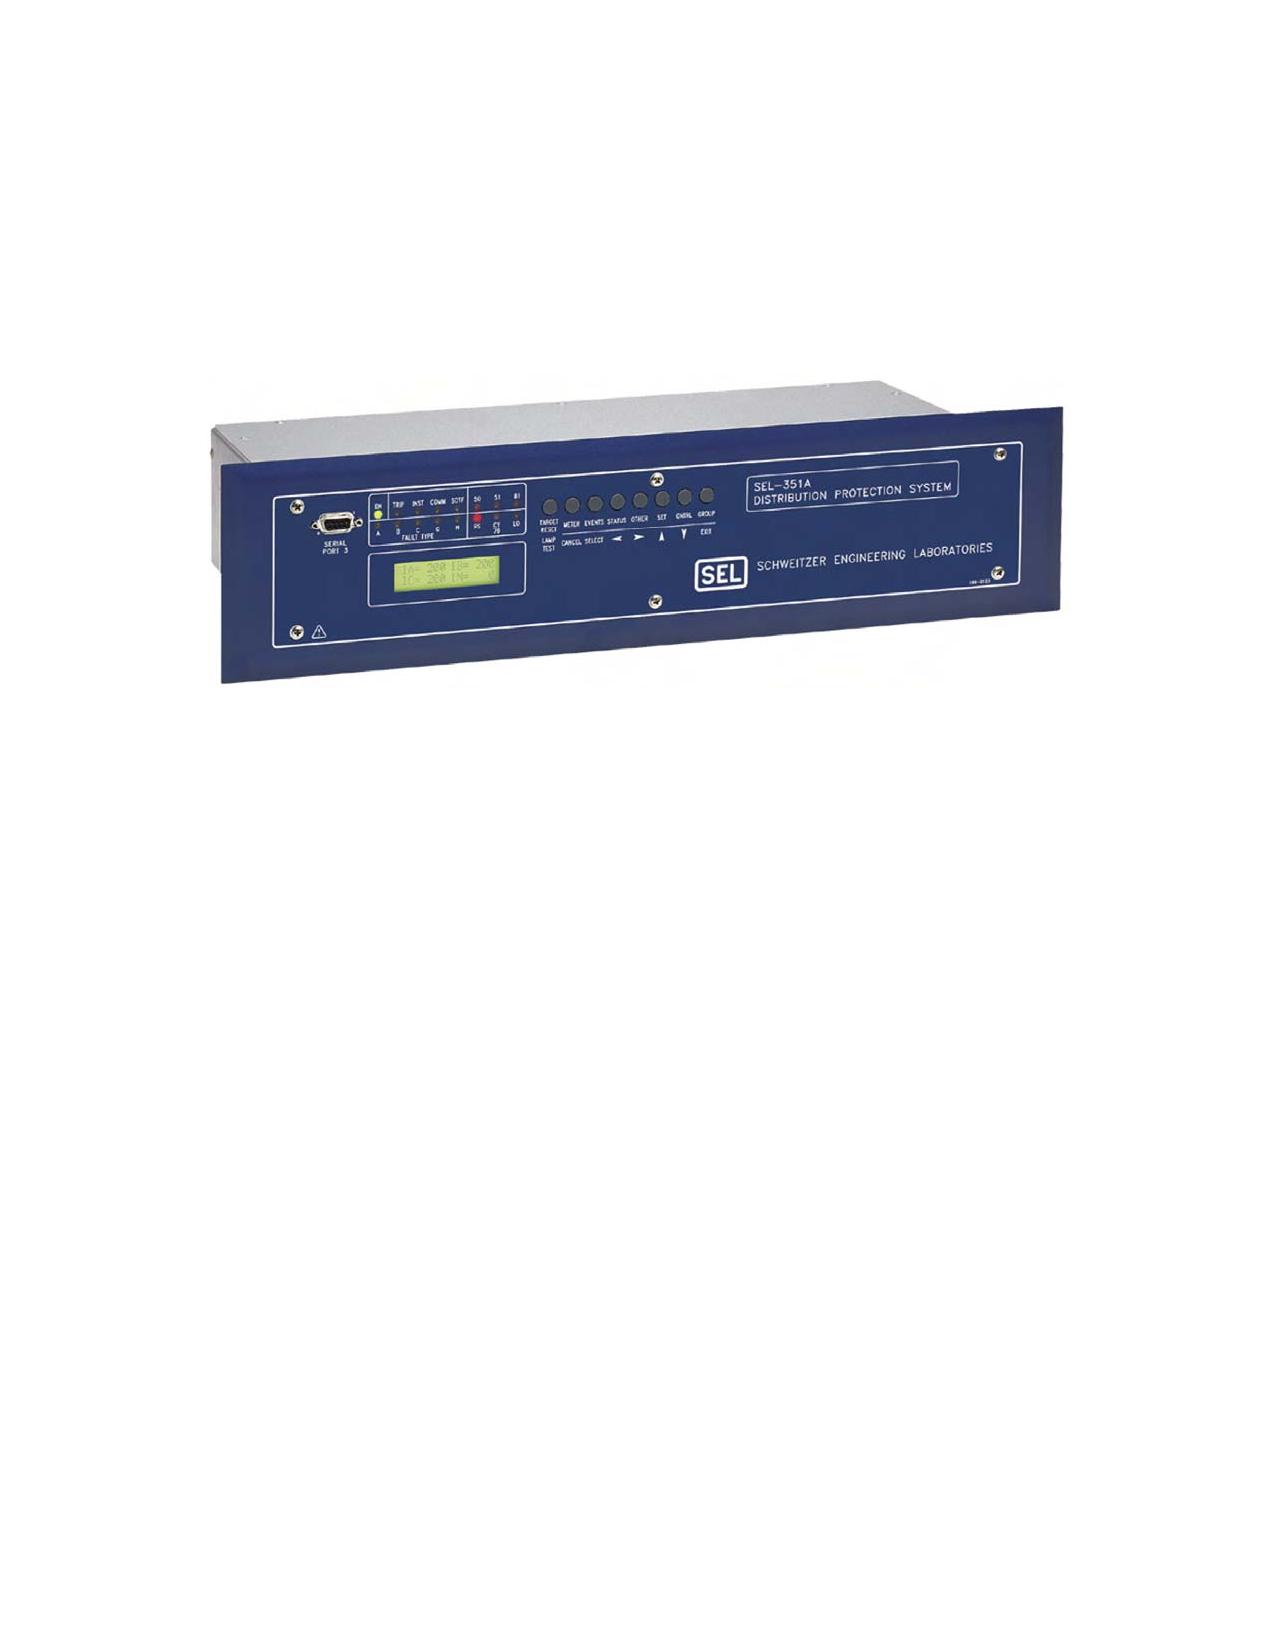
\includegraphics[width=10.8cm]{sel.pdf}
  \legend{Fonte: Do autor}
  \label{fig:rele}
\end{figure}

\begin{longtable}{|l|p{0.8\textwidth}|}
\caption{Tabela ANSI}
 \\ \hline
  Nº & Denominação \\ \hline
  1 & Elemento Principal \\ \hline
  2 & Relé de partida ou fechamento temporizado \\ \hline
  3 & Relé de verificação ou interbloqueio \\ \hline
  4 & Contator principal \\ \hline
  5 & Dispositivo de interrupção \\ \hline
  6 & Disjuntor de partida \\ \hline
  7 & Relé de taxa de variação \\ \hline
  8 & Dispositivo de desligamento da energia de controle \\ \hline
  9 & Dispositivo de reversão \\ \hline
  10 & Chave comutadora de sequência das unidades \\ \hline
  11 & Dispositivo multifunção \\ \hline
  12 & Dispositivo de sobrevelocidade \\ \hline
  13 & Dispositivo de rotação síncrona \\ \hline
  14 & Dispositivo de subvelocidade \\ \hline
  15 & Dispositivo de ajuste ou comparação de velocidade e/ou frequência \\ \hline
  16 & Dispositivo de comunicação de dados \\ \hline
  17 & Chave de derivação ou descarga \\ \hline
  18 & Dispositivo de aceleração ou desaceleração \\ \hline
  19 & Contator de transição partida-marcha \\ \hline
  20 & Válvula operada eletricamente \\ \hline
  21 & Relé de distância \\ \hline
  22 & Disjuntor equalizador \\ \hline
  23 & Dispositivo de controle de temperatura \\ \hline
  24 & Relé de sobreexcitação ou Volts por Hertz \\ \hline
  25 & Relé de verificação de Sincronismo ou Sincronização \\ \hline
  26 & Dispositivo térmico do equipamento \\ \hline
  27 & Relé de subtensão \\ \hline
  28 & Detector de chama \\ \hline
  29 & Contator de isolamento \\ \hline
  30 & Relé anunciador \\ \hline
  31 & Dispositivo de excitação  \\ \hline
  32 & Relé direcional de potência \\ \hline
  33 & Chave de posicionamento \\ \hline
  34 & Dispositivo master de sequência \\ \hline
  35 & Dispositivo para operação das escovas ou curto-circuitar anéis coletores \\ \hline
  36 & Dispositivo de polaridade ou polarização \\ \hline
  37 & Relé de subcorrente ou subpotência \\ \hline
  38 & Dispositivo de proteção de mancal \\ \hline
  39 & Monitor de condições mecânicas \\ \hline
  40 & Relé de perda de excitação ou relé de perda de campo \\ \hline
  41 & Disjuntor ou chave de campo \\ \hline
  42 & Disjuntor / chave de operação normal \\ \hline
  43 & Dispositivo de transferência ou seleção manual \\ \hline
  44 & Relé de sequência de partida  \\ \hline
  45 & Monitor de condições atmosféricas \\ \hline
  46 & Relé de reversão ou desbalanceamento de corrente \\ \hline
  47 & Relé de reversão ou desbalanceamento de tensão \\ \hline
  48 & Relé de sequência incompleta / partida longa \\ \hline
  49 & Relé térmico \\ \hline
  50 & Relé de sobrecorrente instantâneo \\ \hline
  51 & Relé de sobrecorrente temporizado \\ \hline
  52 & Disjuntor de corrente alternada \\ \hline
  53 & Relé para excitatriz ou gerador CC \\ \hline
  54 & Dispositivo de acoplamento \\ \hline
  55 & Relé de fator de potência \\ \hline
  56 & Relé de aplicação de campo \\ \hline
  57 & Dispositivo de aterramento ou curto-circuito \\ \hline
  58 & Relé de falha de retificação \\ \hline
  59 & Relé de sobretensão \\ \hline
  60 & Relé de balanço de corrente ou tensão \\ \hline
  61 & Sensor de densidade \\ \hline
  62 & Relé temporizador \\ \hline
  63 & Relé de pressão de gás (Buchholz) \\ \hline
  64 & Relé detetor de terra \\ \hline
  65 & Regulador \\ \hline
  66 & Relé de supervisão do número de partidas  \\ \hline
  67 & Relé direcional de sobrecorrente  \\ \hline
  68 & Relé de bloqueio por oscilação de potência \\ \hline
  69 & Dispositivo de controle permissivo \\ \hline
  70 & Reostato  \\ \hline
  71 & Dispositivo de detecção de nível \\ \hline
  72 & Disjuntor de corrente contínua \\ \hline
  73 & Contator de resistência de carga \\ \hline
  74 & Relé de alarme \\ \hline
  75 & Mecanismo de mudança de posição \\ \hline
  76 & Relé de sobrecorrente CC \\ \hline
  77 & Dispositivo de telemedição \\ \hline
  78 & Relé de medição de ângulo de fase / proteção contra falta de sincronismo \\ \hline
  79 & Relé de religamento \\ \hline
  80 & Chave de fluxo \\ \hline
  81 & Relé de frequência (sub ou sobre) \\ \hline
  82 & Relé de religamento de carga de CC \\ \hline
  83 & Relé de seleção / transferência automática \\ \hline
  84 & Mecanismo de operação \\ \hline
  85 & Relé receptor de sinal de telecomunicação (teleproteção) \\ \hline
  86 & Relé auxiliar de bloqueio \\ \hline
  87 & Relé de proteção diferencial \\ \hline
  88 & Motor auxiliar ou motor gerador \\ \hline
  89 & Chave seccionadora \\ \hline
  90 & Dispositivo de regulação (regulador de tensão) \\ \hline
  91 & Relé direcional de tensão \\ \hline
  92 & Relé direcional de tensão e potência \\ \hline
  93 & Contator de variação de campo \\ \hline
  94 & Relé de desligamento \\ \hline
  95 & Usado para aplicações específicas  \\ \hline
  96 & Relé auxiliar de bloqueio de barra  \\ \hline
  97 à 99 & Usado para aplicações específicas  \\ \hline
  150 & Indicador de falta à terra  \\ \hline
  AFD & Detector de arco voltaico  \\ \hline
  CLK & Clock  \\ \hline
  DDR & Sistema dinâmico de armazenamento de perturbações  \\ \hline
  DFR & Sistema de armazenamento de faltas digital  \\ \hline
  ENV & Dados do ambiente  \\ \hline
  HIZ & Detector de faltas com alta impedância  \\ \hline
  HMI & Interface Homem-Máquina  \\ \hline
  HST & Histórico  \\ \hline
  LGC & Esquema lógico  \\ \hline
  MET & Medição de Subestação  \\ \hline
  PDC & Concentrador de dados de fasores  \\ \hline
  PMU & Unidade de medição de fasores  \\ \hline
  PQM & Esquema de monitoramento de potência  \\ \hline
  RIO & Dispositivo Remoto de Inputs/Outputs  \\ \hline
  RTU & Unidade de terminal remoto / Concentrador de Dados  \\ \hline
  SER & Sistema de armazenamento de eventos  \\ \hline
  TCM & Esquema de monitoramento de Trip  \\ \hline
  SOTF & Fechamento sob falta  \\ \hline
\end{longtable}


\subsubsection*{Complementação da Tabela ANSI:}
50N - sobrecorrente instantâneo de neutro\par
51N - sobrecorrente temporizado de neutro ( tempo definido ou curvas inversas)\par
50G - sobrecorrente instantâneo de terra (comumente chamado 50GS)\par
51G - sobrecorrente temporizado de terra (comumente chamado 51GS e com tempo definido ou curvas inversas)\par
50BF - relé de proteção contra falha de disjuntor (também chamado de 50/62 BF)\par
51Q - relé de sobrecorrente temporizado de seqüência negativa com tempo definido ou curvas inversas\par
51V - relé de sobrecorrente com restrição de tensão\par
51C - relé de sobrecorrente com controle de torque\par
50PAF - sobrecorrente de fase instantânea de alta velocidade para detecção de arco voltaico\par
50NAF - sobrecorrente de neutro instantânea de alta velocidade para detecção de arco voltaico\par
59Q - relé de sobretensão de seqüência negativa\par
59N - relé de sobretensão residual ou sobretensão de neutro (também chamado de 64G) , calculado ou TP em delta aberto
64 - relé de proteção de terra pode ser por corrente ou por tensão. Os diagramas unifilares devem indicar se este elemento é alimentado por TC ou por TP, para que se possa definir corretamente. Se for alimentado por TC, também pode ser utilizado como uma unidade 51 ou 61. Se for alimentado por TP, pode-se utilizar uma unidade 59N ou 64G. A função 64 também pode ser encontrada como proteção de carcaça, massa-cuba ou tanque, sendo aplicada em transformadores de força até 5 MVA.\par
67N - relé de sobrecorrente direcional de neutro (instantâneo ou temporizado)\par
67G - relé de sobrecorrente direcional de terra (instantâneo ou temporizado)\par
67Q - relé de sobrecorrente direcional de seqüência negativa\par
78 - Salto vetorial (Vector Shift)\par

\subsubsection*{Proteção Diferencial - ANSI 87:}
O relé diferencial 87 pode ser de diversas maneiras:\par
87T - diferencial de transformador (pode ter 2 ou 3 enrolamentos)\par
87N - diferencial de neutro\par
REF – falta restrita à terra\par
87Q - diferencial de sequência negativa (aplicado para detecção de faltas entre espiras em transformadores)\par
87G - diferencial de geradores\par
87GT - proteção diferencial do grupo gerador-transformador\par
87SP - proteção diferencial de fase dividida de geradores\par
87V – Diferencial de tensão de fase\par
87VN – Diferencial de tensão de neutro\par
87B - diferencial de barras. Pode ser de alta, média ou baixa impedância\par
Pode-se encontrar em circuitos industriais elementos de sobrecorrente ligados num esquema diferencial, onde os TCs de fases são somados e ligados ao relé de sobrecorrente.\par
Também encontra-se um esquema de seletividade lógica para realizar a função diferencial de barras.\par
Pode-se encontrar em algumas documentações o relé 68 sendo referido à função de seletividade lógica.\par
87M - diferencial de motores - Neste caso pode ser do tipo percentual ou do tipo autobalanceado.\par
O percentual utiliza um circuito diferencial através de 3 TCs de fases e 3 TCs no neutro do motor. O tipo autobalanceado utiliza um jogo de 3 TCs nos terminais do motor, conectados de forma à obter a somatória das correntes de cada fase e neutro. Na realidade, trata-se de um elemento de sobrecorrente, onde o esquema é diferencial e não o relé.\par

\subsubsection*{Dispositivo de comunicação de dados - ANSI 16:}
As letras sufixos ao dispositivo definem sua aplicação. Os primeiros sufixos são:\par
S – comunicação de dados serial\par
E – comunicação de dados Ethernet\par
Os sufixos subsequentes definem:\par
C – dispositivo de segurança de rede (ex. VPN, encriptação)\par
F – firewall ou filtro de mensagens\par
M – função de gerenciamento da rede (SNMP)\par
R – roteador\par
S – switch\par
T – telefone\par
Uma switch Ethernet gerenciável terá o seguinte código: 16ESM\par

\section{Anunciadores de Alarme}
Anunciadores de alarme têm como principal função sinalizar corretamente estados críticos de instalações, preservando a integridade das mesmas. Eles sinalizam acústica e oticamente alarmes de equipamentos numa forma padronizada, dentro do mais elevado padrão ergonômico e cognitivo possível. Recomenda-se, em geral, realizar a conexão direta de sinais elétricos de alarme do campo com o anunciador, evitando-se a sua passagem por sistemas digitais de automação e de controle. Assim, obtém-se um nível de segurança operacional adequado.\par
O comprimento máximo de cabos de sinal é de 600 m (sem blindagem) ou de 1000 m (com blindagem). Estes valores máximos podem ser fortemente reduzidos em áreas com fortes campos eletromagnéticos, como em calhas a céu aberto em subestações. Também é de suma importância que os cabos sejam alocados em calhas portando cabos com tensões homogêneas. A alocação de cabos de alta e baixa tensão conjuntamente em calhas pode causar disfunções sérias no anunciador ou mesmo falhas de hardware.\par

\begin{figure}[htb]
  \caption{Anunciadores de alarmes SEL-2523}
  \centering
  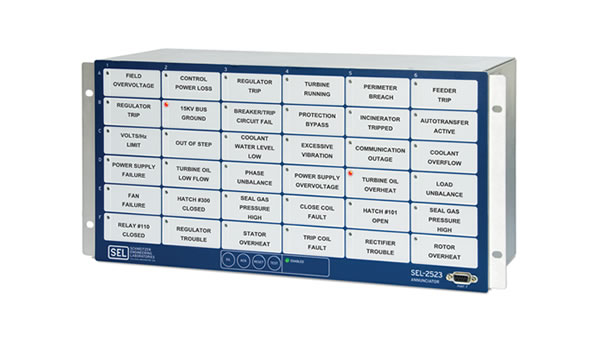
\includegraphics[width=10.8cm]{anunciador.jpg}
% \legend{Fonte: Do autor}
  \label{fig:anunciador}
\end{figure}




% ---------------------------------------------------
% Capítulo 2
% ---------------------------------------------------

\chapter{Projeto de subestações de alta tensão}
\label{chap:projSEAT}
\lipsum

% ---------------------------------------------------
% Capítulo 3
% ---------------------------------------------------

\chapter{Problemática da Demanda de Carga da Subestação Camboriú (CBU) -- SC}
\label{chap:demCarga}
\lipsum

% ---------------------------------------------------
% Capítulo 4
% ---------------------------------------------------

\chapter{Solução de Ampliação para a Subestação Camboriú}
\label{chap:solAmp}
\lipsum

% ---------------------------------------------------
% Capítulo 5
% ---------------------------------------------------

\chapter{Como é feito em outras partes do mundo}
\label{chap:asbuiltAbroad}
\lipsum


% ---------------------------------------------------
% Conclusão
% ---------------------------------------------------
\chapter*[Conclusão]{Conclusão}
\addcontentsline{toc}{chapter}{Conclusão}
\lipsum


\bibliography{refs}
\end{document}



%\begin{figure}[htb]
%	\caption{Sinal de ECG}
%	\centering
%	\includegraphics[width=16cm]{matlab1.pdf}
%	\legend{Fonte: Do autor}
%	\label{fig:matlab1}
%\end{figure}

